% =======================================================
% 7. FLUSSO DEI DATI (DATA FLOW)
% =======================================================
\section{Flusso dei Dati (Data Flow)}
Questa sezione illustra il ciclo di vita delle informazioni all'interno del sistema, partendo dall'interazione dell'utente fino all'ottenimento del risultato generato dall'AI o alla persistenza della nota. 

Le frecce continue con punta piena rappresentano chiamate sincrone, le frecce tratteggiate le risposte (reply), le frecce continue con punta stilizzata rappresentano chiamate asincrone, infine, quelle contrassegnate \guillemotleft create\guillemotright\ istanziano un nuovo oggetto comando. I riquadri tratteggiati etichettati \texttt{alt} rappresentano rami alternativi mutuamente esclusivi, ciascuno introdotto da una guardia tra parentesi quadre (es. \texttt{[range definito]}): solo il ramo la cui condizione è verificata viene eseguito.
\subsection{Elaborazione di un'operazione AI}
Il flusso, dalla richiesta dell’utente alla visualizzazione della proposta, attraversa tre diagrammi di sequenza in successione, ciascuno con una responsabilità netta: il primo e il terzo rimangono all’interno del Frontend (rispettivamente l’avvio della richiesta e la ricezione della risposta), mentre il secondo descrive l’intero tratto di rete dal Frontend verso il Backend e l’LLM esterno.

\paragraph*{1a -- Richiesta operazione AI (tratto Frontend).} Il flusso ha inizio quando l’Utente seleziona una porzione di testo all'interno dell'editor e richiede un'operazione specifica (ad esempio, cliccando su "Riassumi"). Questa interazione viene catturata direttamente dal componente di View \texttt{AIPanelView}, che aggiorna il proprio stato registrando la richiesta nell'oggetto \texttt{lastRequestedOperation} ed eseguendo una \texttt{notify()} locale per aggiornare la visualizzazione. La notifica viene intercettata dal controller AIController tramite il metodo \texttt{update()}, il quale interroga la View tramite \texttt{getLastRequestedOperation()} per recuperare i dati dell'operazione. Il controller esegue la propria logica interna tramite \texttt{onAIRequest()} e richiama il metodo \texttt{requestAIOperation(type, text)} esposto da \texttt{AIRequestModel}. A questo punto, il Model imposta il proprio stato interno (aiState) su Processing e si auto-notifica, propagando l'aggiornamento a tutti gli observer registrati. AIPanelView intercetta la notifica \texttt{update()}, interroga lo stato tramite \texttt{getAIState()}, e, ricevendo la variante \texttt{ProcessingState}, mostra immediatamente all'utente uno spinner visivo di caricamento e l'opzione per consentire l'interruzione manuale (R72-F-O, R73-F-O). In parallelo, \texttt{AIRequestModel} avvia la richiesta asincrona di elaborazione verso il server richiamando il metodo \texttt{requestOperation(type, text)} del componente di infrastruttura \texttt{AIServiceProxy}.

\begin{figure}[H]
	\centering
	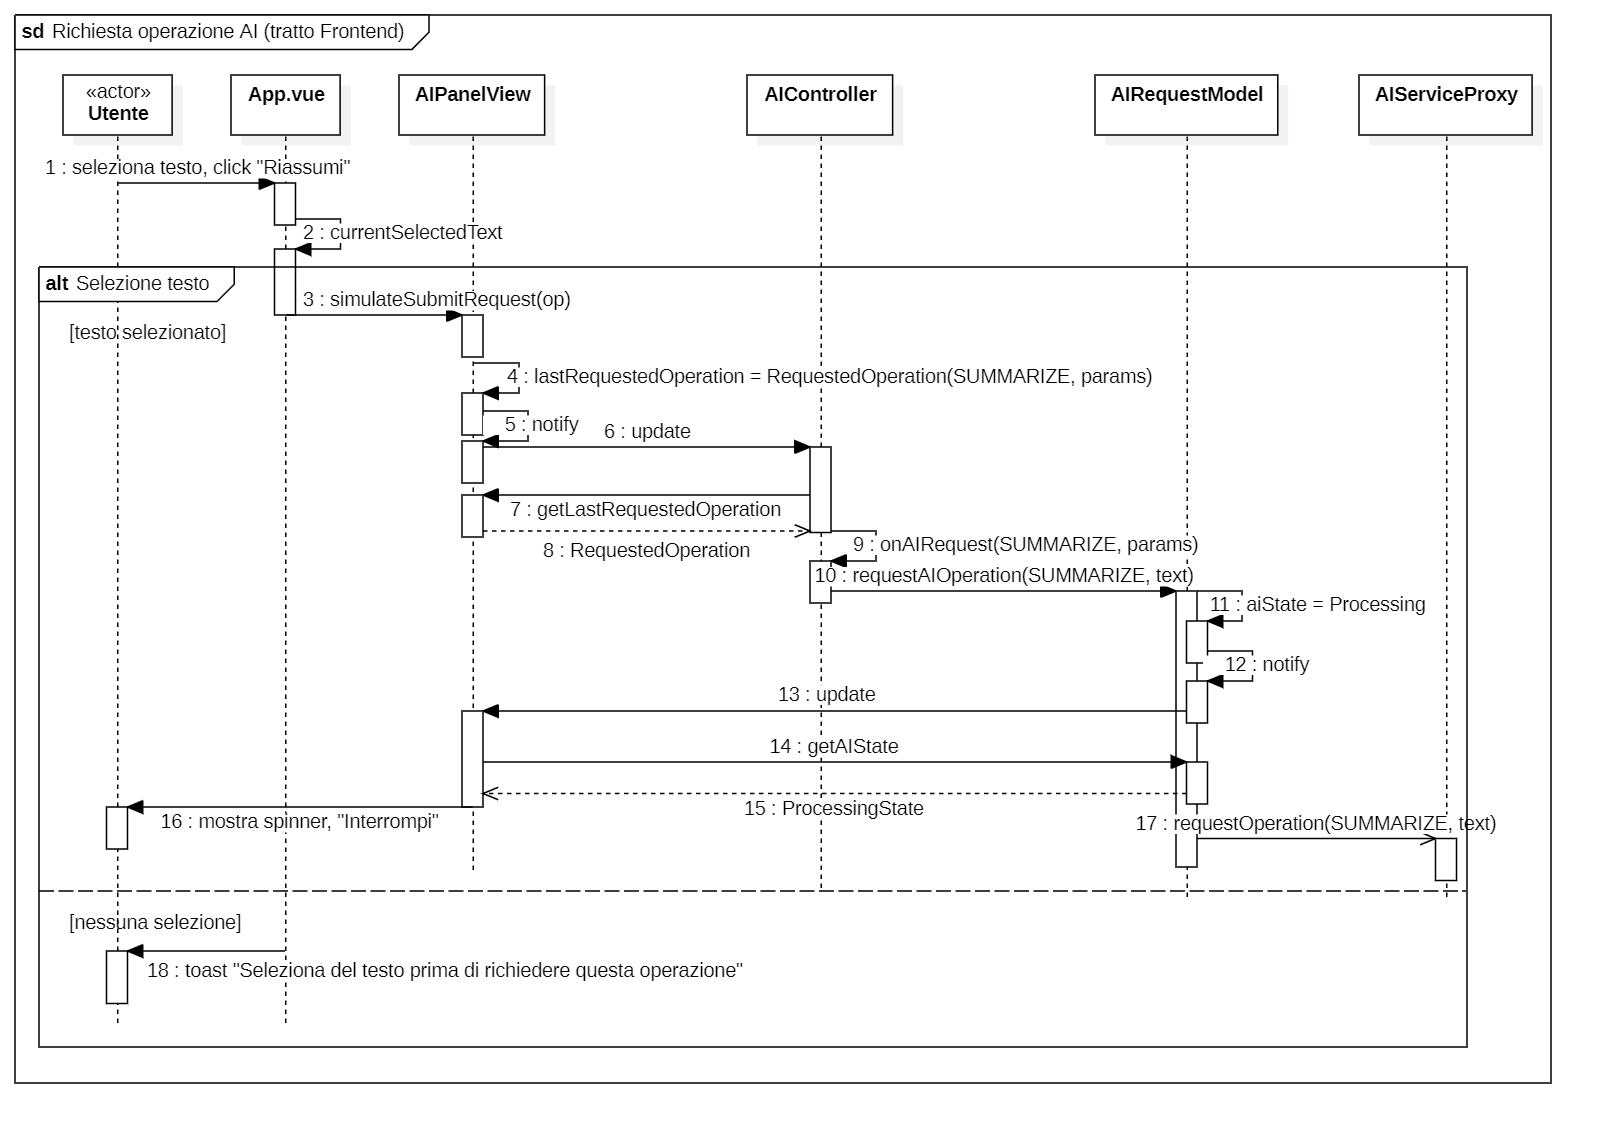
\includegraphics[width=0.9\textwidth]{diagrammi/diagrammi_sequenze/richiesta_op_ai_frontend.png}
	\caption{Richiesta operazione AI (tratto Frontend).}
	\label{fig:seq-1a}
\end{figure}

\paragraph*{1b -- Richiesta AI (tratto REST→LLM).} \texttt{AIRouter} riceve la richiesta e la inoltra ad \texttt{AIService}, che risolve la strategia corretta tramite la Simple Factory e costruisce un \texttt{Prompt} tramite \texttt{PromptBuilder}. La chiamata attraversa poi il decorator di logging fino all'\texttt{OpenAIAdapter}, che contatta il servizio LLM esterno; la risposta risale la stessa catena fino a \texttt{AIService}, che costruisce la \texttt{Proposal} e la restituisce come \texttt{AIOperationResponse}.

\begin{figure}[H]
	\centering
	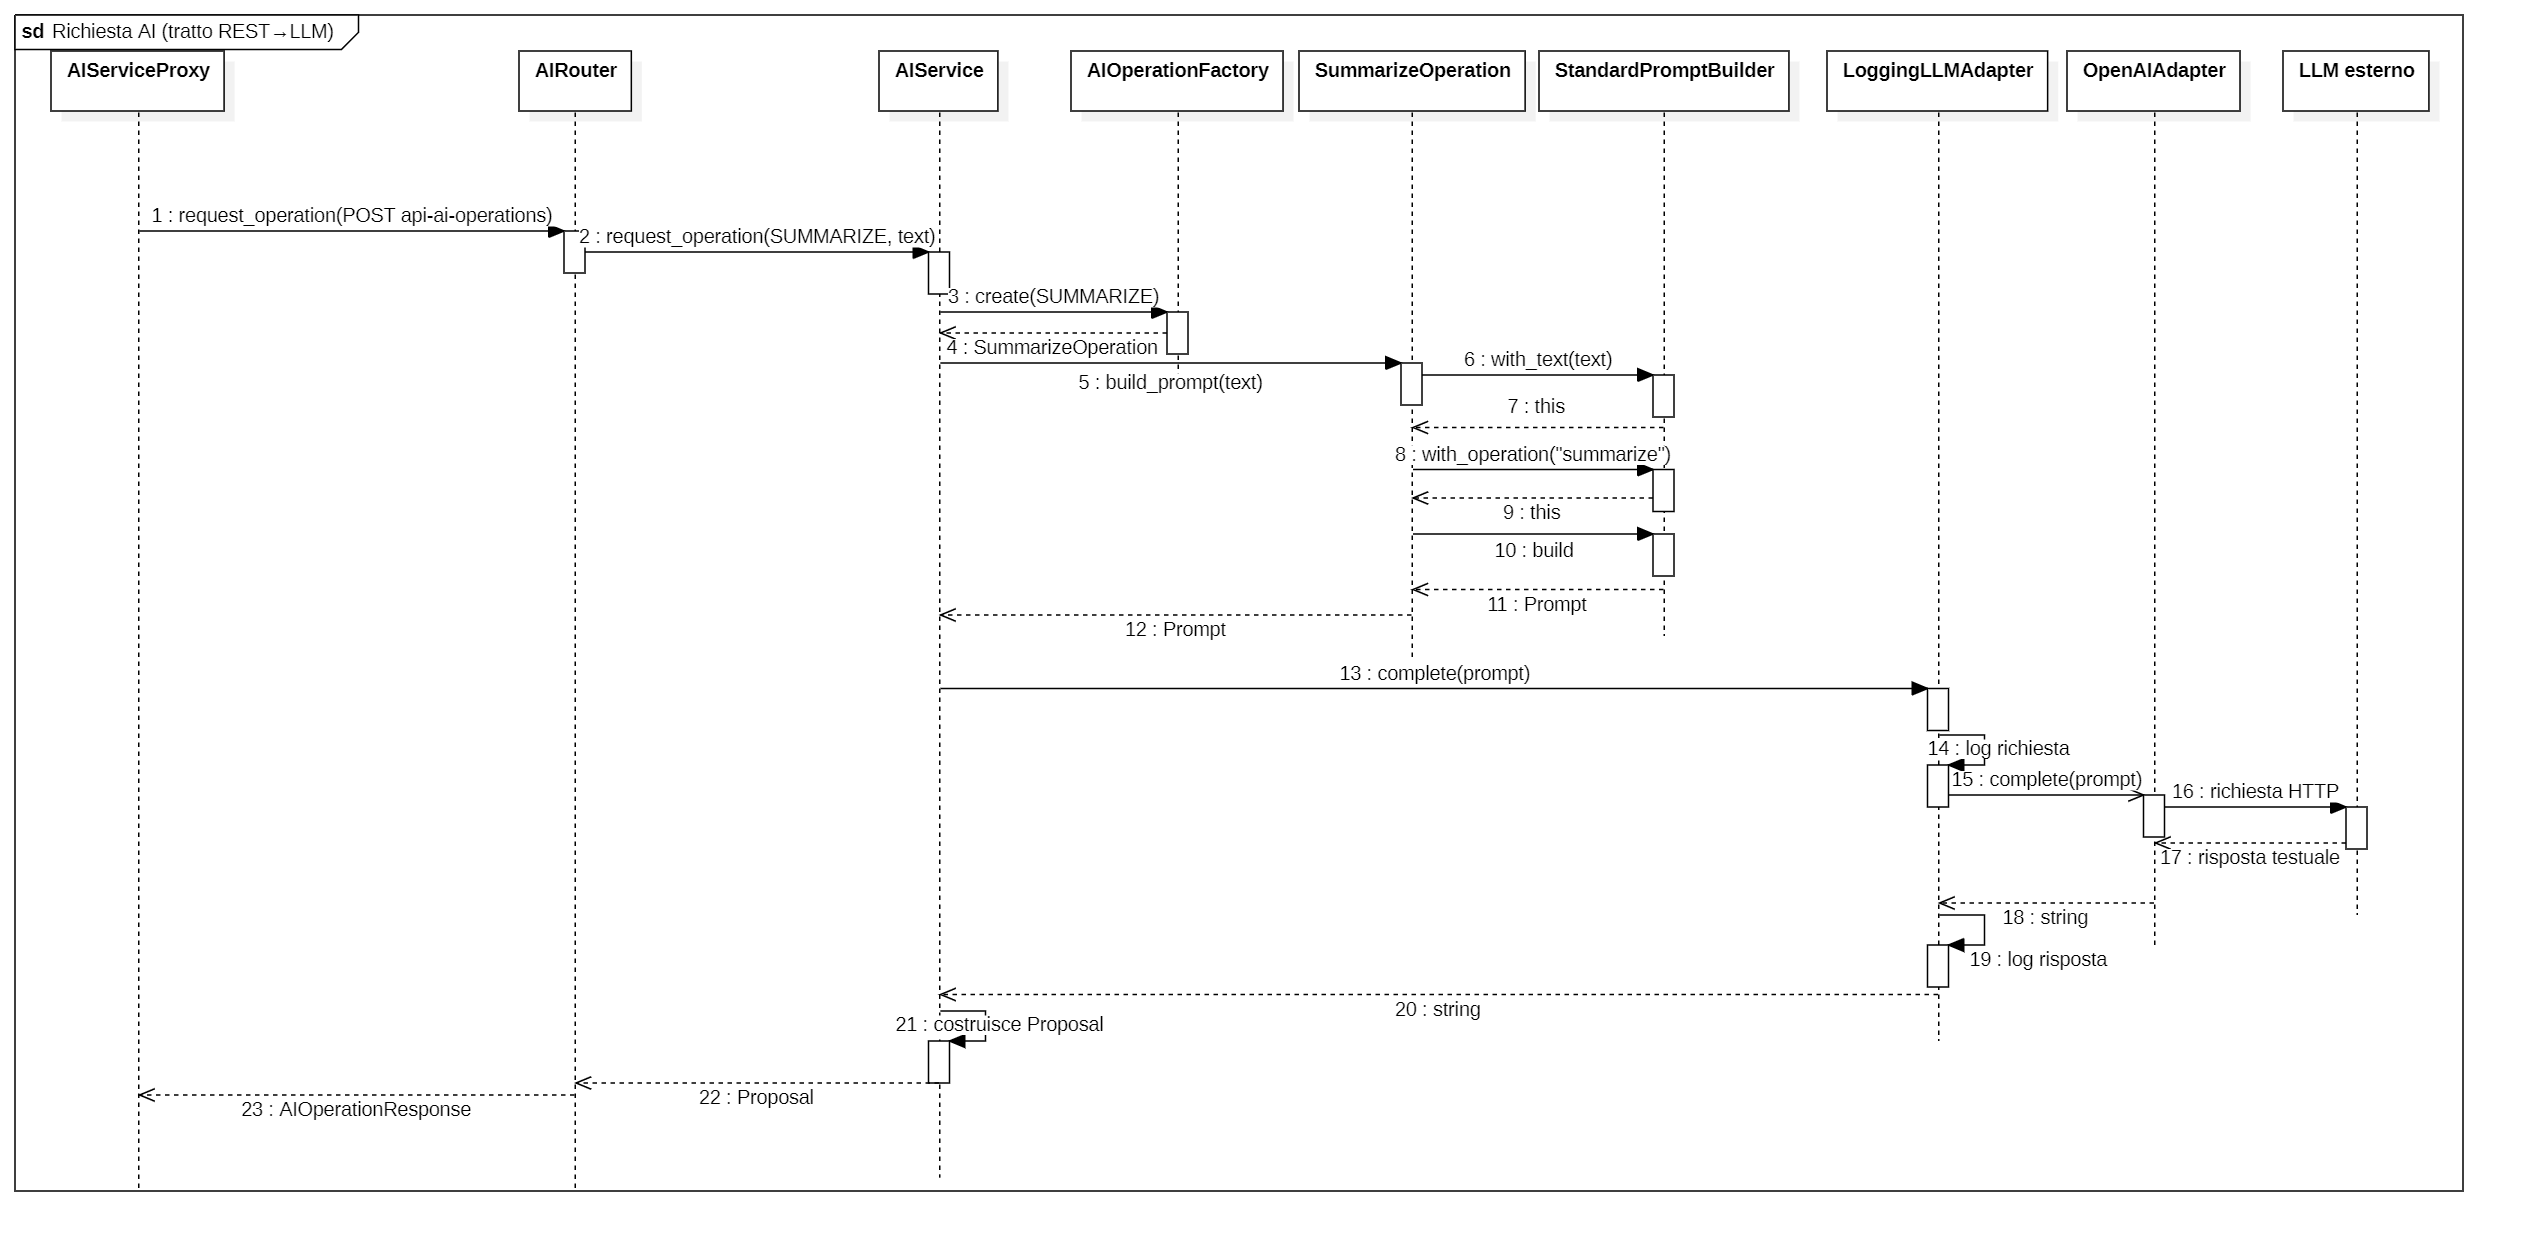
\includegraphics[width=\textwidth]{diagrammi/diagrammi_sequenze/richiesta_ai_backend.png}
	\caption{Richiesta AI (tratto REST→LLM): attraversa in un unico flusso i pattern Strategy, Builder, Simple Factory, Decorator e Adapter.}
	\label{fig:seq-1b}
\end{figure}

\paragraph*{1c -- Ricezione proposta AI (tratto Frontend).} La risposta HTTP, una volta risolta la Promise di \texttt{AIServiceProxy.requestOperation()}, riporta il controllo al Model: \texttt{AIRequestModel} transita allo stato \texttt{ProposalReadyState(proposal)} e notifica gli observer; \texttt{AIPanelView} interroga lo stato aggiornato e mostra all'utente la proposta con le azioni disponibili (Accetta/Rifiuta/Rigenera).

\begin{figure}[H]
	\centering
	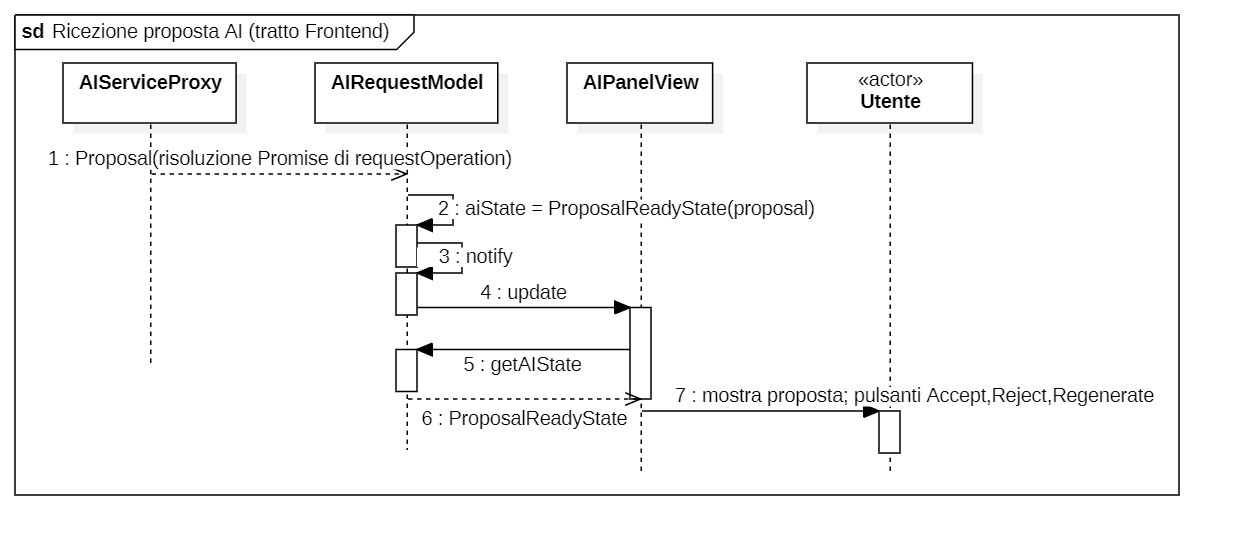
\includegraphics[width=\textwidth]{diagrammi/diagrammi_sequenze/ricezione_proposta_frontend.png}
	\caption{Ricezione proposta AI (tratto Frontend).}
	\label{fig:seq-1c}
\end{figure}

\FloatBarrier

\subsection{Gestione della proposta AI ed elenco delle operazioni}
\paragraph*{Accetta proposta AI (riuso Command).} Se l'utente accetta la proposta, \texttt{AIController} recupera lo stato da \texttt{AIRequestModel} (\texttt{ProposalReadyState}) e sceglie il comando in base alla presenza del range originario della selezione, tramite un frame \texttt{alt}: nel ramo normale (\texttt{[range definito]}, praticamente sempre) crea un \texttt{ReplaceContentCommand} che sostituisce il testo selezionato con la proposta; nel ramo di rete di sicurezza (\texttt{[range non definito]}, es. una selezione persa nel frattempo) crea invece un \texttt{InsertTextCommand} che inserisce la proposta in coda al documento. In entrambi i casi il comando è eseguito tramite \\ \texttt{NoteModel.executeCommand()}. Il Model torna quindi allo stato \texttt{Idle} e il pannello proposta si chiude.

\begin{figure}[H]
	\centering
	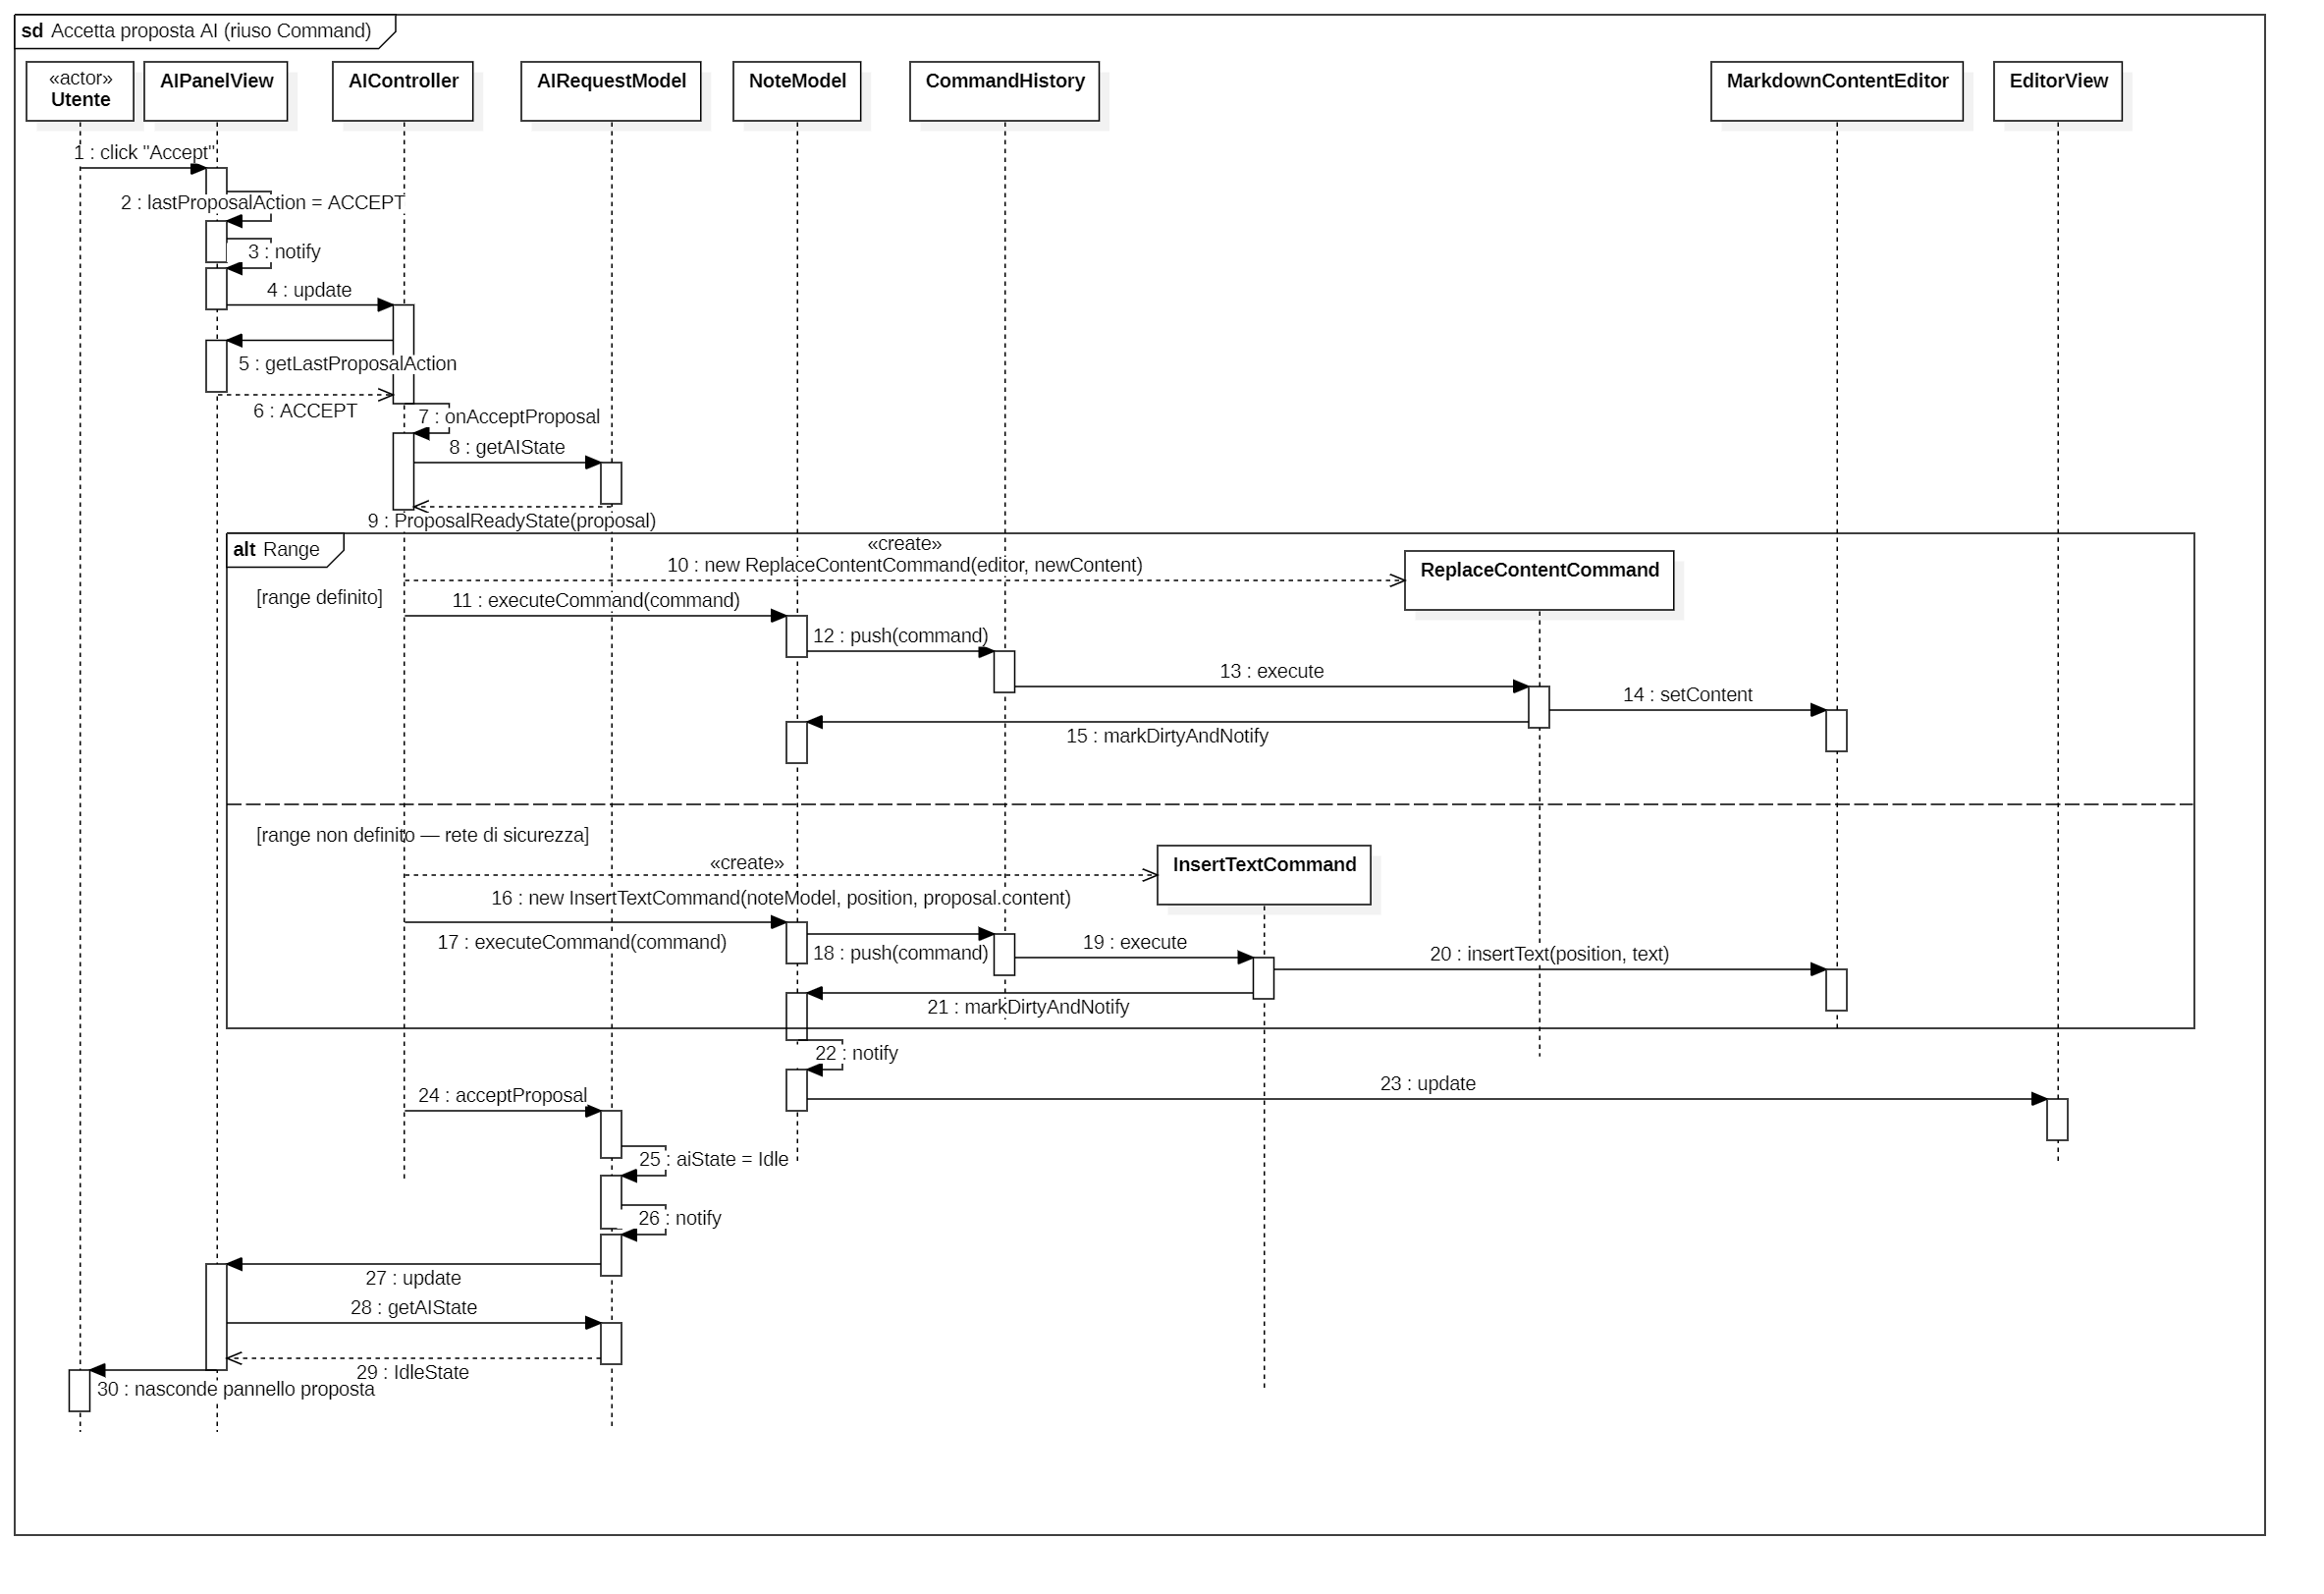
\includegraphics[width=\textwidth]{diagrammi/diagrammi_sequenze/accetta_proposta.png}
	\caption{Accetta proposta AI (riuso del pattern Command): \texttt{ReplaceContentCommand} nel ramo normale, \texttt{InsertTextCommand} come rete di sicurezza.}
	\label{fig:seq-accetta}
\end{figure}

\paragraph*{Rifiuta / Rigenera / Interrompi proposta AI.} Le altre tre azioni disponibili sulla proposta condividono lo stesso punto di ingresso (\texttt{AIController.update()}) e si distinguono in un unico frame \texttt{alt} a tre rami: \texttt{Rifiuta} riporta semplicemente il Model a \texttt{Idle} senza toccare il documento; \texttt{Rigenera} ripete la stessa richiesta memorizzata (\texttt{lastRequest}) invocando di nuovo \texttt{requestAIOperation()} -- non esiste un metodo dedicato di rigenerazione sul Model, si riusa lo stesso flusso della richiesta iniziale (Figura~\ref{fig:seq-1a}); \texttt{Interrompi} incrementa un contatore di generazione (\texttt{requestGeneration}) prima di tornare a \texttt{Idle}, così un'eventuale risposta dell'LLM arrivata in ritardo per la richiesta ormai abbandonata viene riconosciuta come obsoleta e ignorata.

\begin{figure}[H]
	\centering
	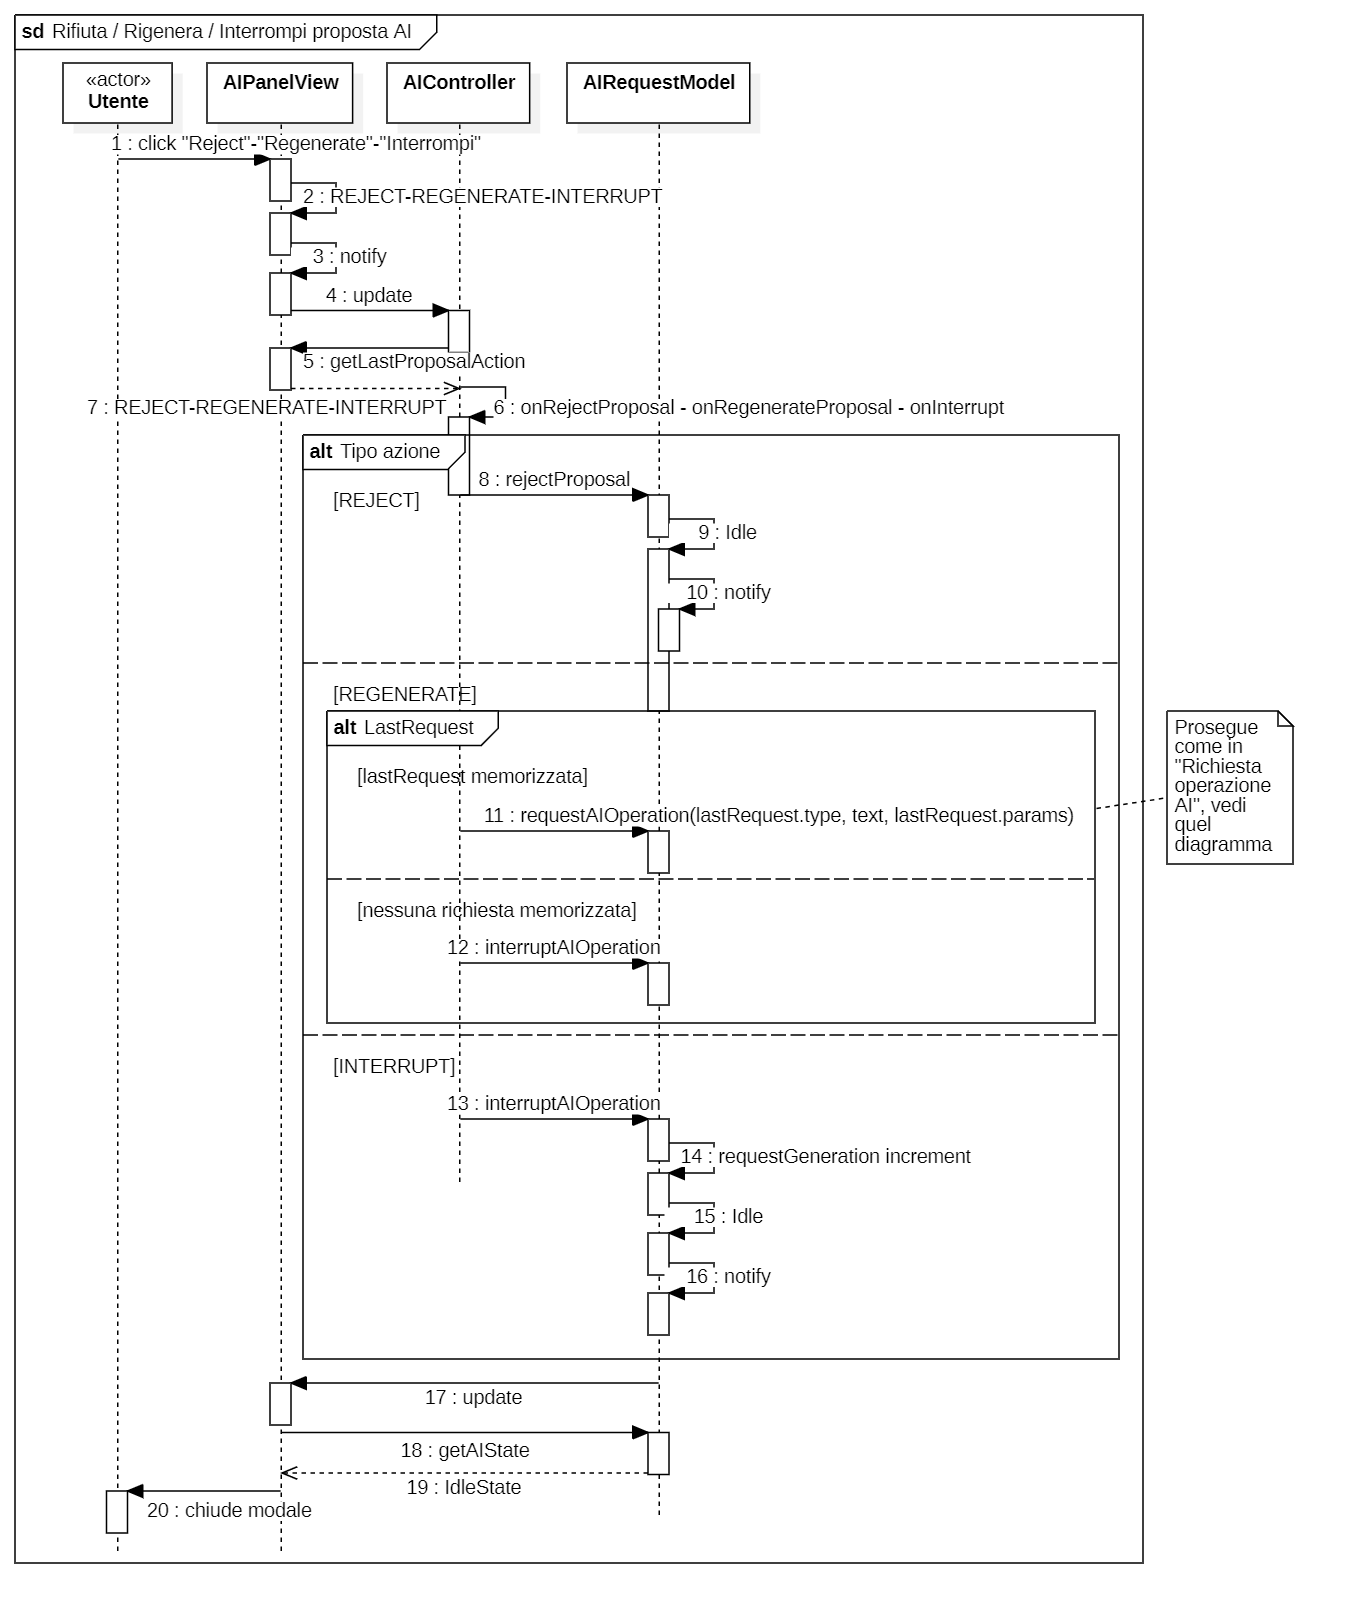
\includegraphics[width=0.9\textwidth]{diagrammi/diagrammi_sequenze/gestione_proposta_ai.png}
	\caption{Rifiuta, Rigenera e Interrompi la proposta AI (frame \texttt{alt} a tre rami).}
	\label{fig:seq-gestione-proposta}
\end{figure}

\paragraph*{Elenco operazioni disponibili (Simple Factory self-registration).} L'elenco delle operazioni mostrate nel selettore del Frontend non è hard-coded: \texttt{AIPanelView} lo richiede a runtime, risalendo la catena fino ad \texttt{AIOperationFactory.available\_types()}, che legge il proprio registro di auto-registrazione. Aggiungere una nuova operazione AI non richiede quindi alcuna modifica a questo flusso.

\begin{figure}[H]
	\centering
	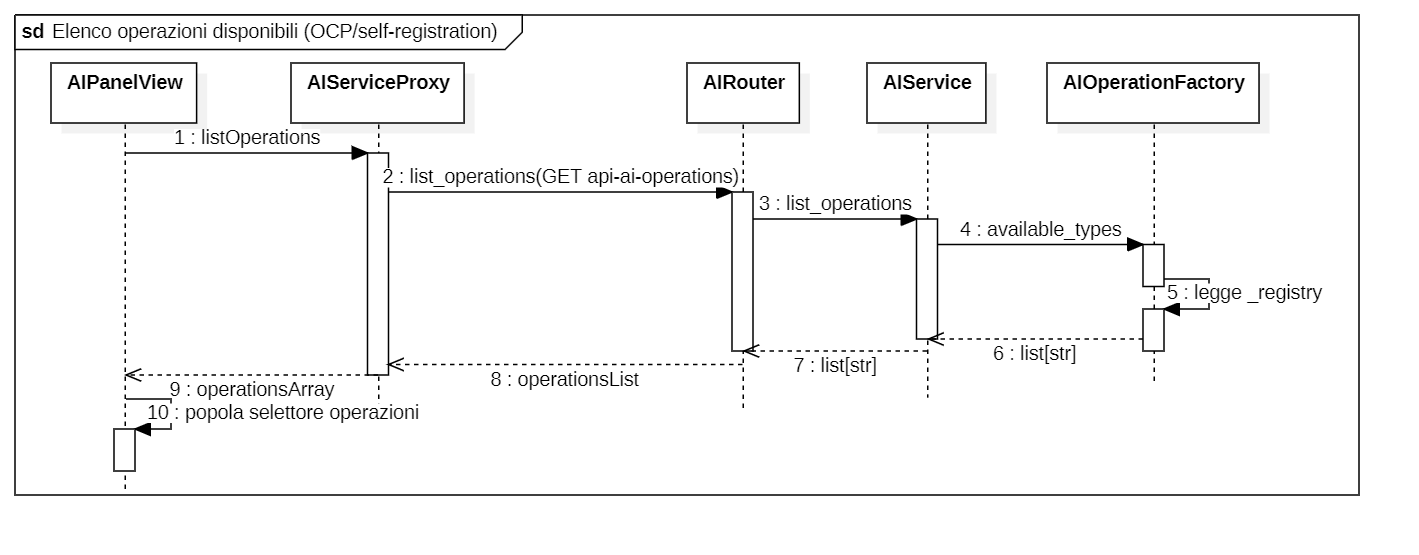
\includegraphics[width=0.85\textwidth]{diagrammi/diagrammi_sequenze/elenco_operazioni.png}
	\caption{Elenco operazioni disponibili (Simple Factory self-registration).}
	\label{fig:seq-elenco}
\end{figure}

\FloatBarrier

\subsection{Editing del testo e Undo/Redo}
I tre diagrammi seguenti mostrano il riuso dello stesso meccanismo Command/CommandHistory per operazioni di editing diverse (formattazione, tabelle) e per il relativo undo/redo.

\paragraph*{Formattazione con Undo.} La View registra la richiesta dell'utente (es. ``Grassetto''), si auto-notifica, il Controller la preleva e crea il \texttt{FormatTextCommand} corrispondente, eseguito e archiviato da \texttt{CommandHistory}. L'Undo riesegue in ordine inverso l'ultimo comando in pila, ripristinando il contenuto precedente tramite lo stesso oggetto comando.

\begin{figure}[H]
	\centering
	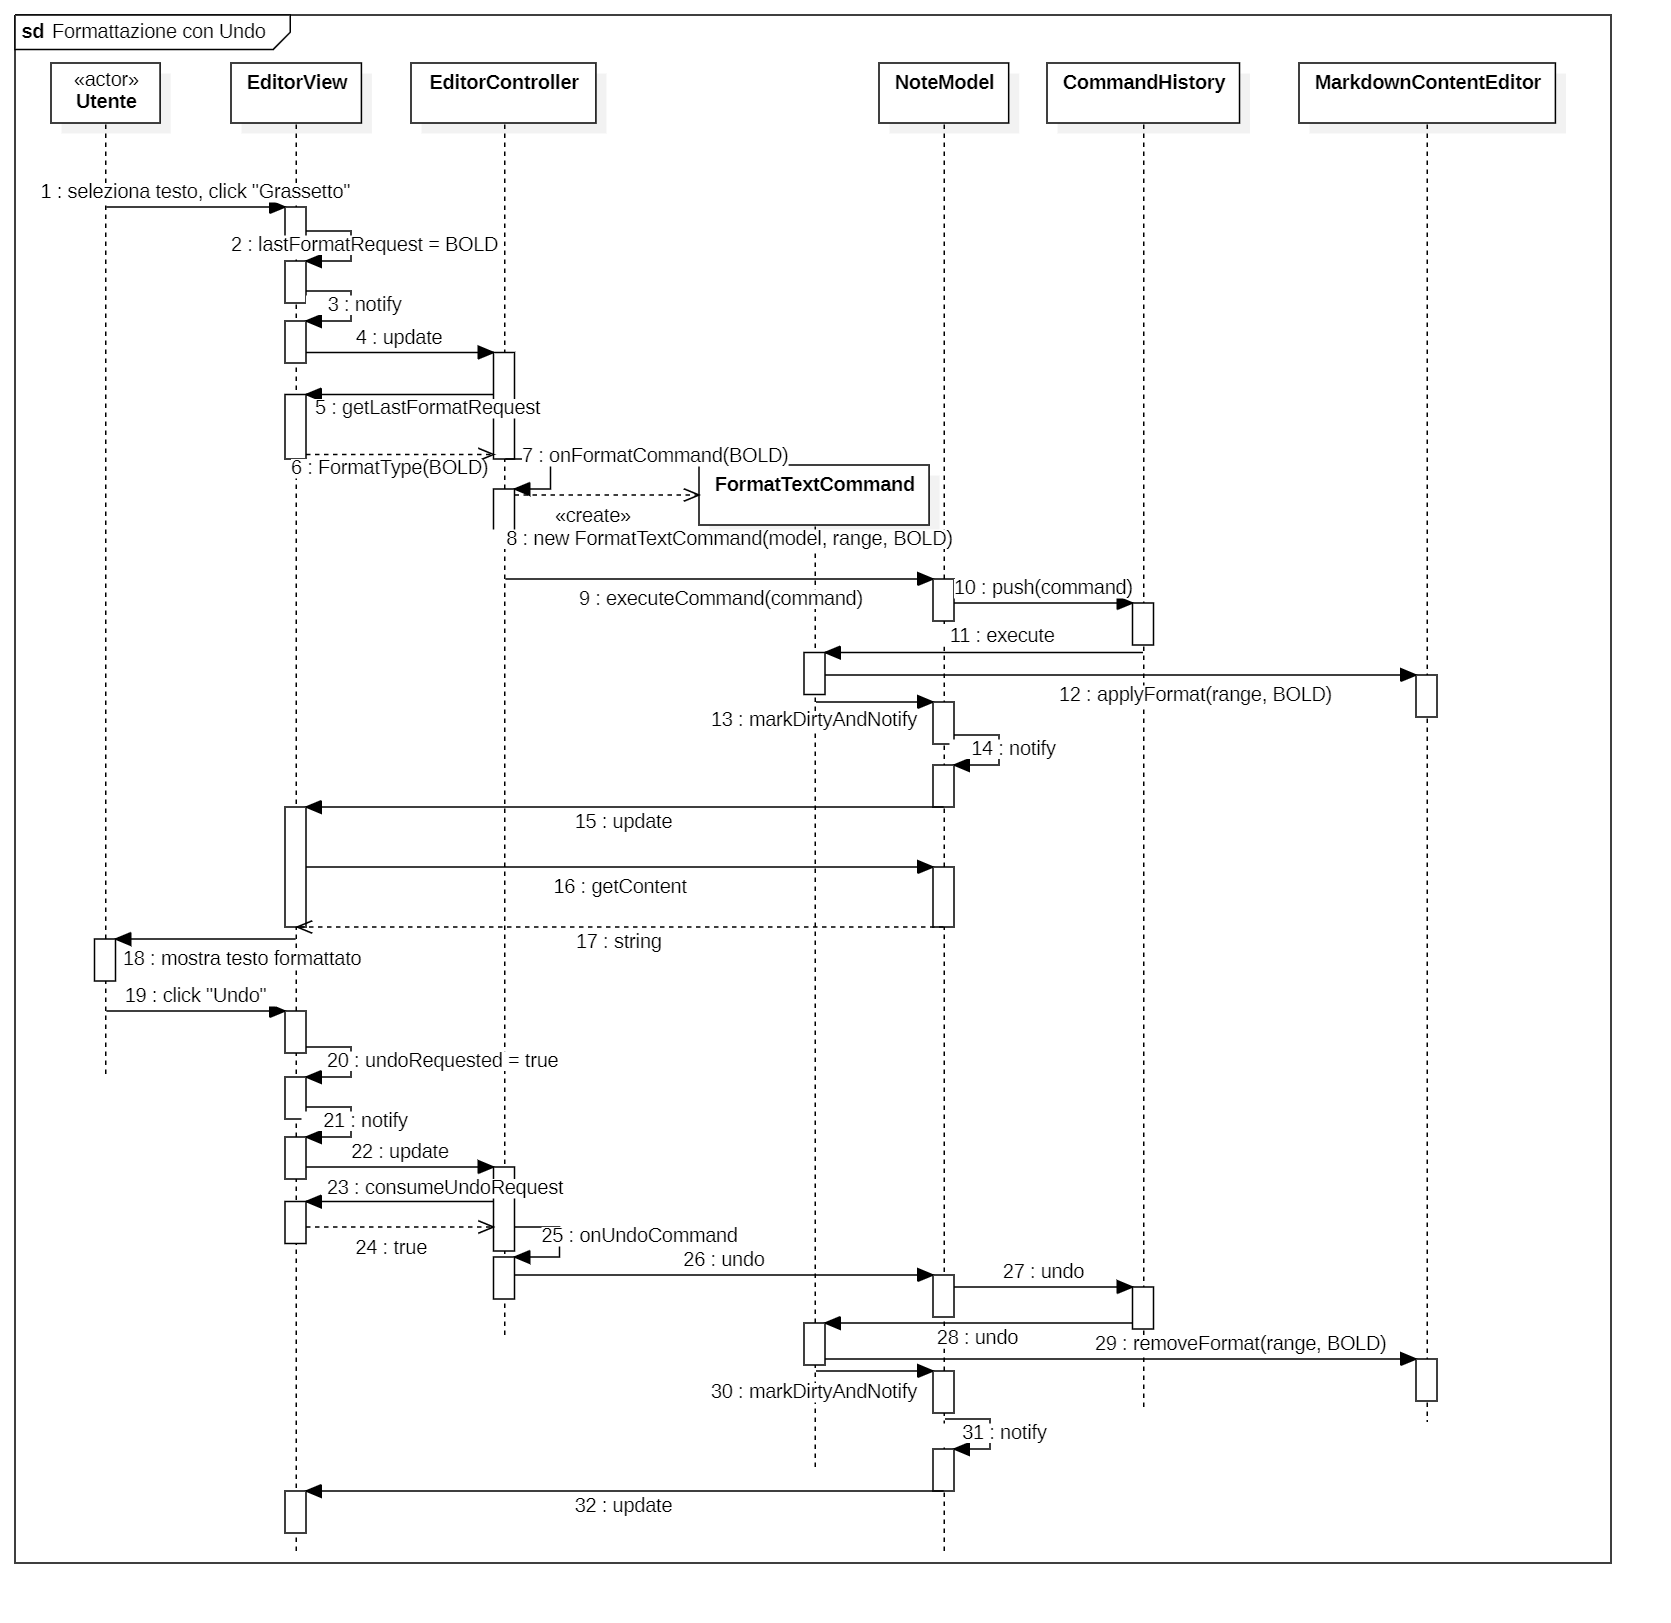
\includegraphics[width=0.9\textwidth]{diagrammi/diagrammi_sequenze/formattazione_undo.png}
	\caption{Formattazione di un testo e relativo Undo.}
	\label{fig:seq-undo}
\end{figure}

\paragraph*{Redo.} Continuazione dello scenario precedente: il Redo rieseguono l'ultimo comando spostato dalla pila di redo a quella di undo.

\begin{figure}[H]
	\centering
	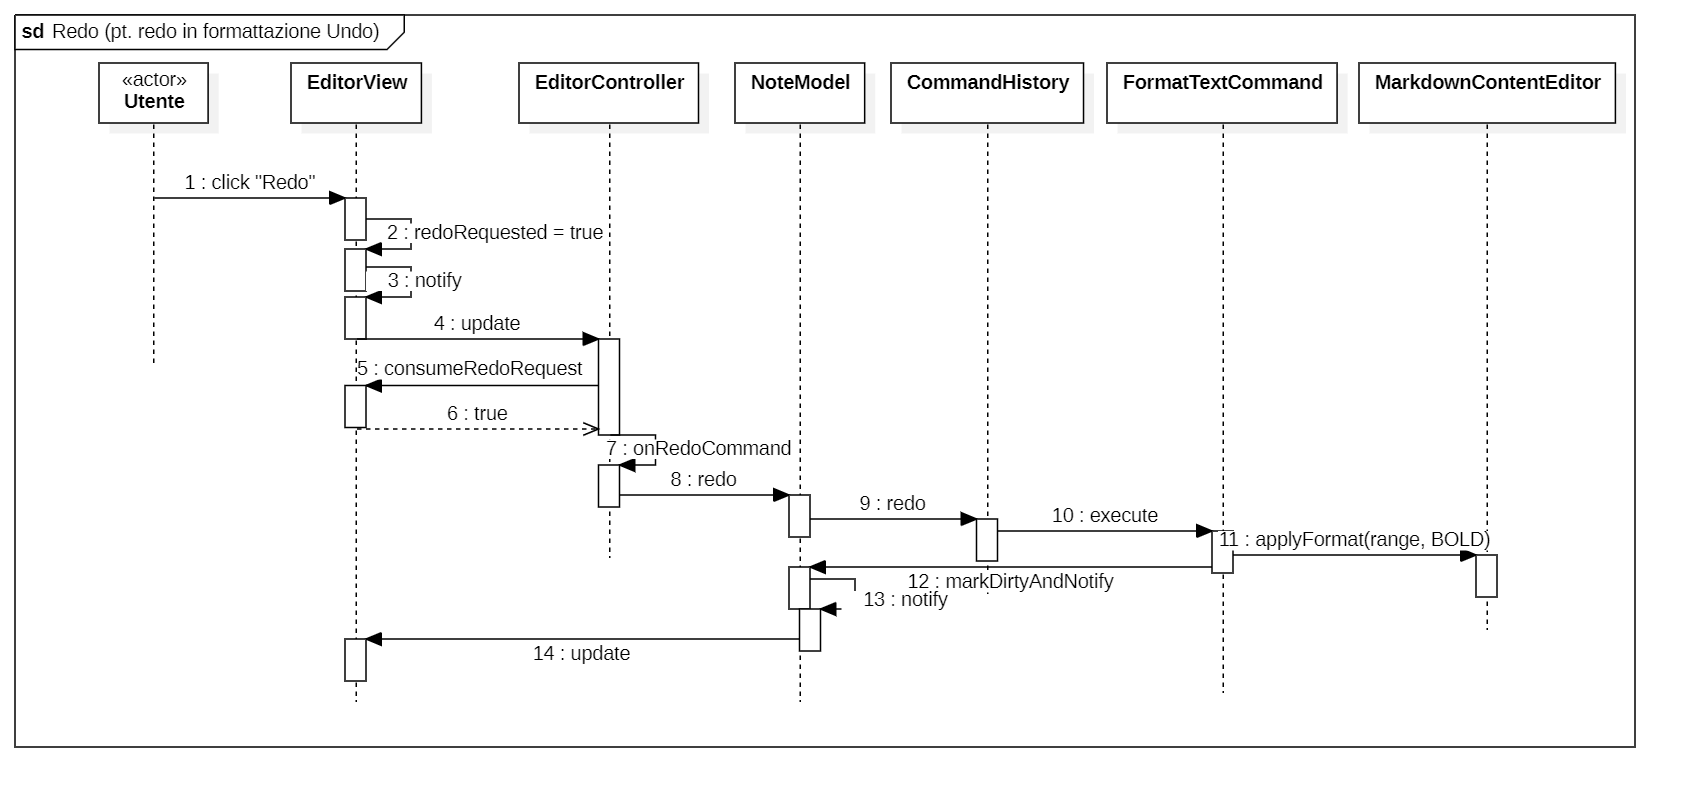
\includegraphics[width=0.85\textwidth]{diagrammi/diagrammi_sequenze/formattazione_redo.png}
	\caption{Redo (continuazione di ``Formattazione con Undo'').}
	\label{fig:seq-redo}
\end{figure}

\paragraph*{Inserimento tabella con validazione.} Il frame \texttt{alt} distingue due rami alternativi: se le dimensioni richieste (righe/colonne) non sono valide, \texttt{MarkdownContentEditor} solleva \\ \texttt{InvalidTableDimensionError}, propagato fino alla View che mostra l'errore senza modificare il documento; se le dimensioni sono valide, la tabella viene inserita e la nota aggiornata normalmente.

\begin{figure}[H]
	\centering
	
\includegraphics[width=\textwidth]{diagrammi/diagrammi_sequenze/inserimento_tabella.png}
	\caption{Inserimento di una tabella, con validazione delle dimensioni.}
	\label{fig:seq-tabella}
\end{figure}

\paragraph*{Copia / Taglia / Incolla.} Le tre operazioni sugli appunti condividono lo stesso frame \texttt{alt} esterno a tre rami, ciascuno con un ulteriore controllo interno sulla presenza di una selezione (Copia, Taglia) o sul permesso di lettura degli appunti concesso dal browser (Incolla): in assenza di selezione o di permesso, l'operazione si conclude con un avviso, senza modificare il documento. Taglia e Incolla, quando vanno a buon fine, riusano \texttt{ReplaceContentCommand} -- lo stesso comando generico impiegato per raggruppare in un'unica voce di \texttt{CommandHistory} le sequenze di digitazione libera -- invece di introdurre comandi dedicati.

\begin{figure}[H]
	\centering
	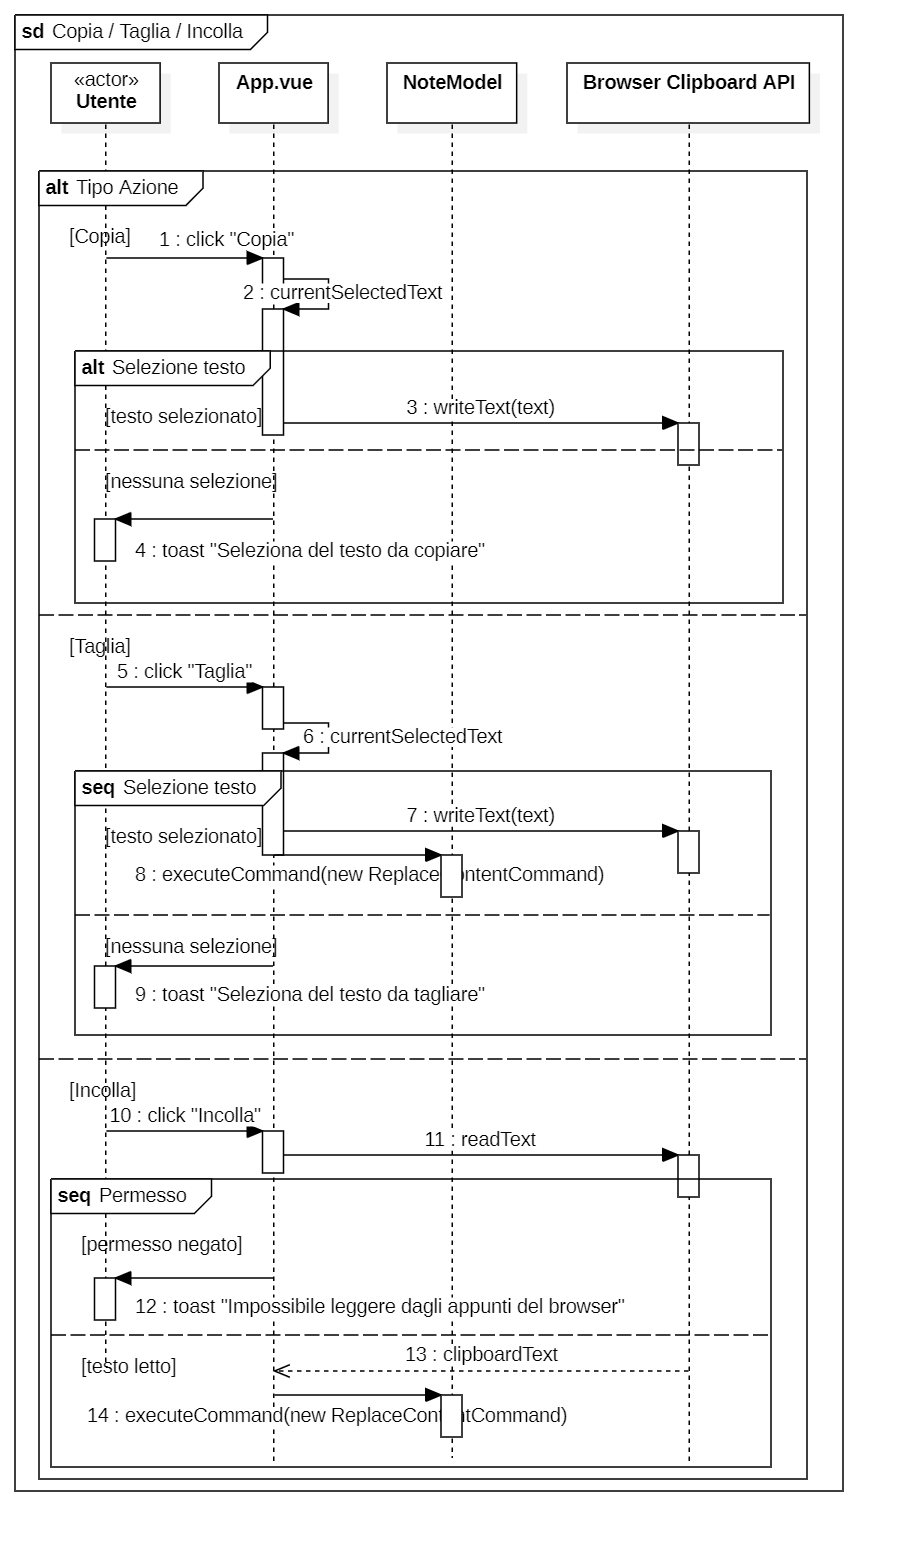
\includegraphics[width=0.9\textwidth]{diagrammi/diagrammi_sequenze/copia_taglia_incolla.png}
	\caption{Copia, Taglia e Incolla (frame \texttt{alt} a tre rami).}
	\label{fig:seq-clipboard}
\end{figure}

\FloatBarrier

\subsection{Persistenza locale della nota}
\paragraph*{Salvataggio nota locale.} Un primo frame \texttt{alt} distingue il salvataggio in base al supporto della File System Access API da parte del browser: se supportata (Chrome, Edge), \texttt{NoteServiceProxy} apre il selettore nativo (\texttt{showSaveFilePicker}) al primo salvataggio e riusa l'handle ottenuto per i successivi; se non supportata (Firefox, Safari -- R5-V-O), ricade su un fallback basato su download (\texttt{Blob} + elemento \texttt{<a download>}), chiedendo il nome del file una sola volta per nota tramite un prompt nativo e riproponendolo nei salvataggi successivi.

\begin{figure}[H]
	\centering
	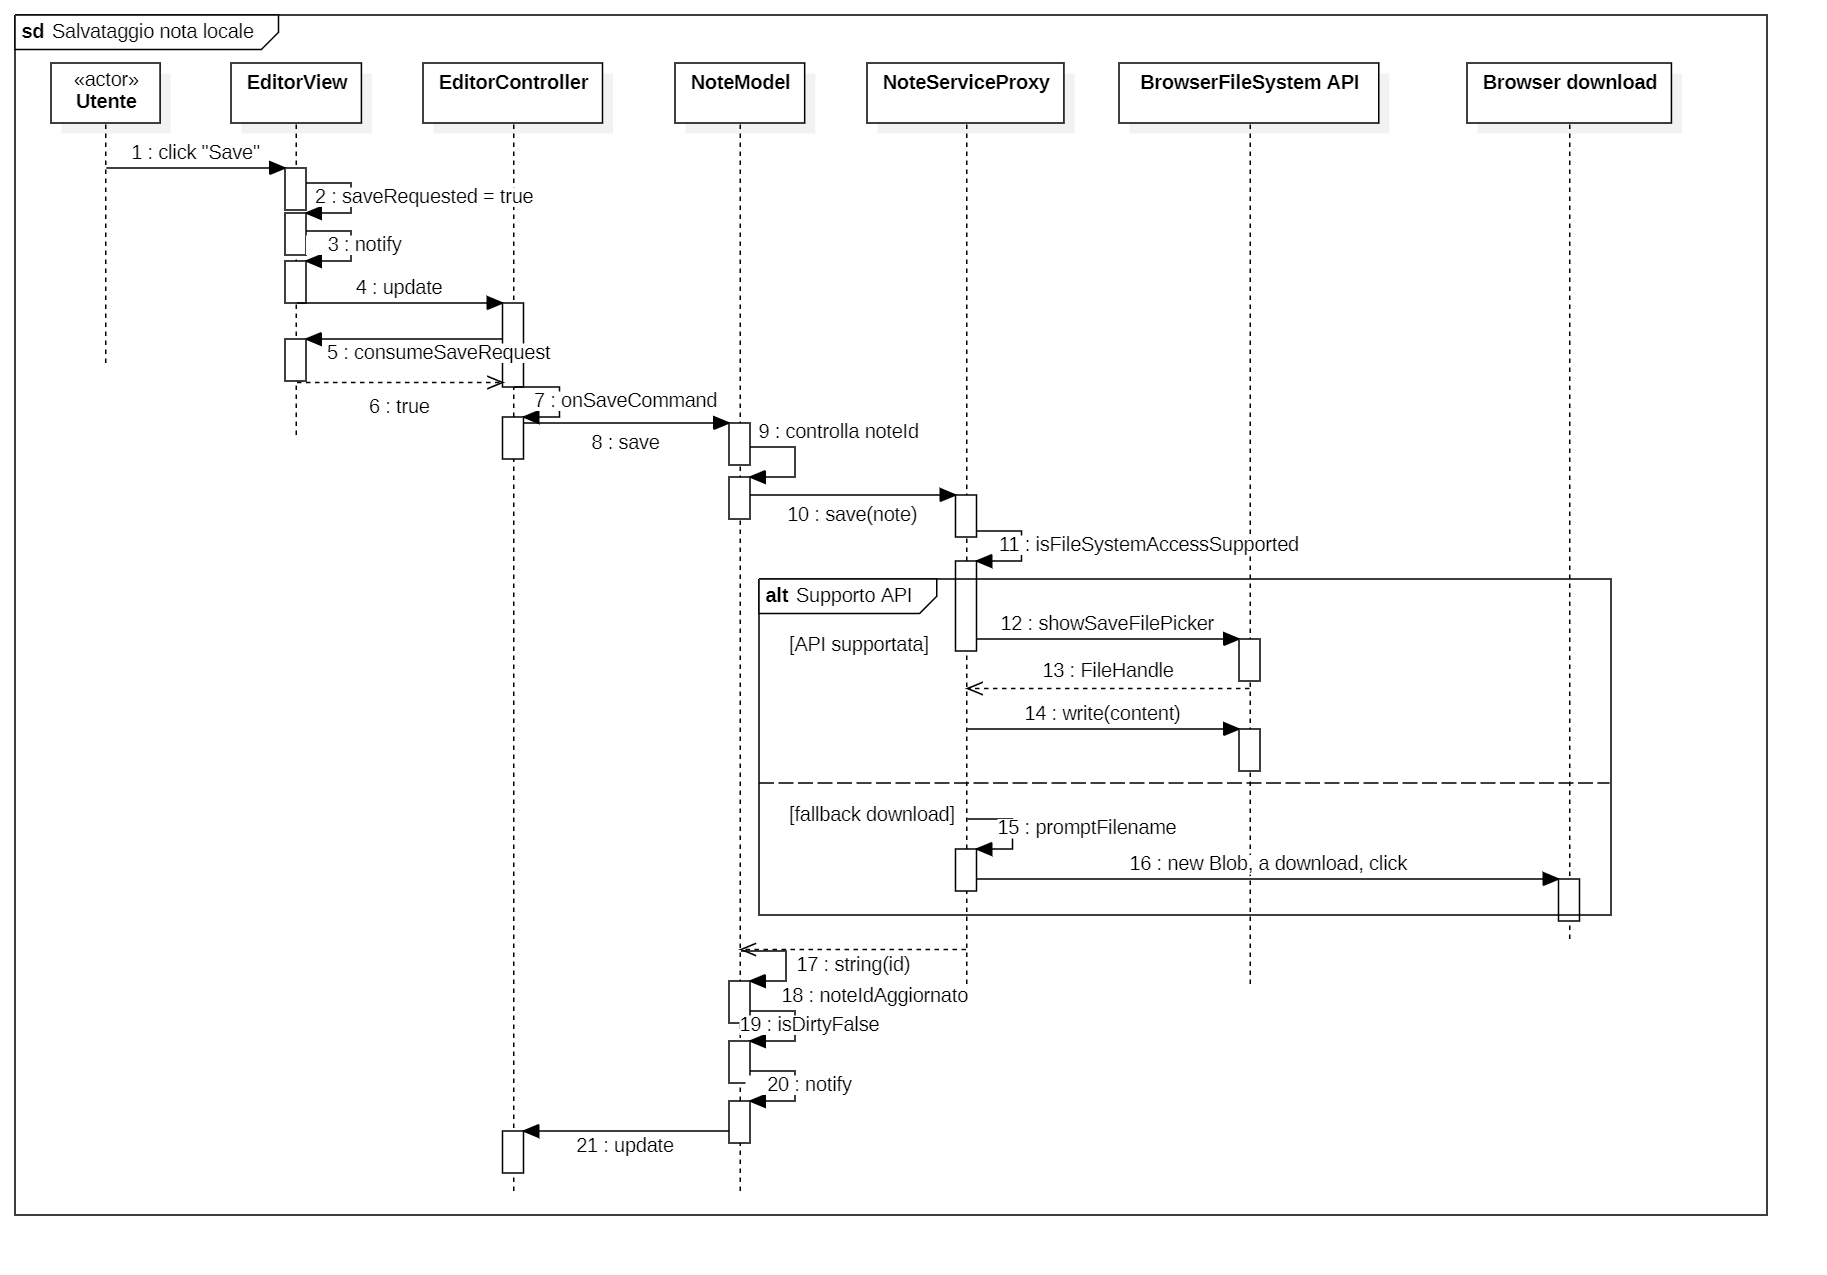
\includegraphics[width=\textwidth]{diagrammi/diagrammi_sequenze/salvataggio_nota.png}
	\caption{Salvataggio di una nota in locale.}
	\label{fig:seq-salvataggio}
\end{figure}

\paragraph*{Salvataggio con errore.} In caso di errore di I/O durante la scrittura, l'eccezione \texttt{NoteIOError} risale da \texttt{BrowserFileSystemAPI} fino alla View, che notifica l'utente mantenendo la nota invariata.

\begin{figure}[H]
	\centering
	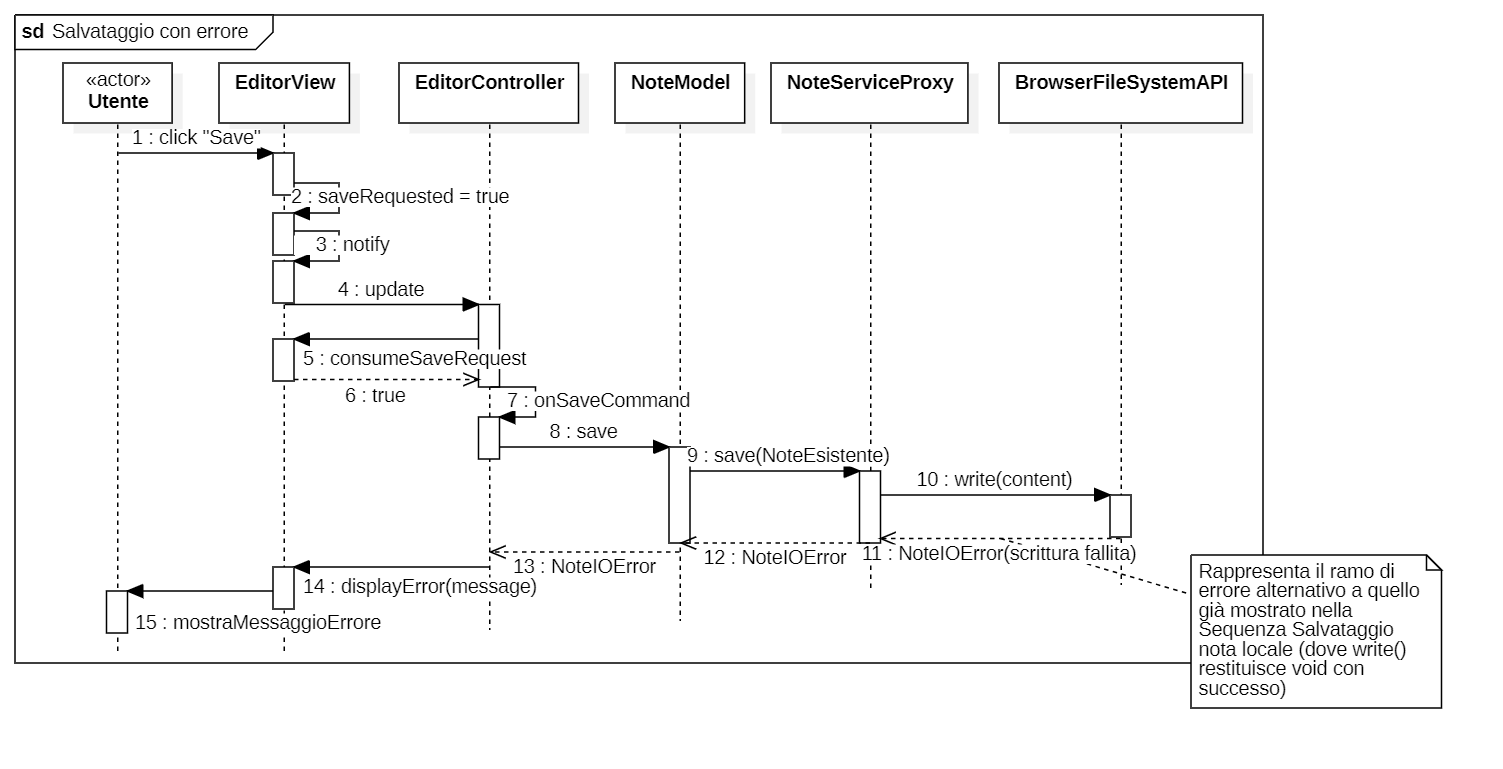
\includegraphics[width=0.85\textwidth]{diagrammi/diagrammi_sequenze/salvataggio_con_errore.png}
	\caption{Salvataggio con errore di I/O.}
	\label{fig:seq-salvataggio-errore}
\end{figure}

\paragraph*{Importazione/Apertura nota.} Analogamente al salvataggio, un frame \texttt{alt} distingue il supporto della File System Access API: se supportata, l'apertura passa dal selettore nativo del browser (\texttt{showOpenFilePicker}), la lettura del contenuto, la ricostruzione dell'oggetto \texttt{Note} e l'aggiornamento di \texttt{MarkdownContentEditor}; la \texttt{CommandHistory} viene azzerata per non permettere un Undo o Redo che attraversino note diverse. Se non supportata (R76-F-O, R5-V-O), il fallback usa un elemento \texttt{<input type="file">} nascosto: un frame \texttt{alt} interno distingue il caso in cui l'utente sceglie un file da quello in cui annulla il selettore -- rilevato tramite il rientro del focus sulla finestra, in assenza di un evento \texttt{cancel} affidabile su tutti i browser -- che produce un \texttt{NoteIOError} con \texttt{cancelled=true}.

\begin{figure}[H]
	\centering
	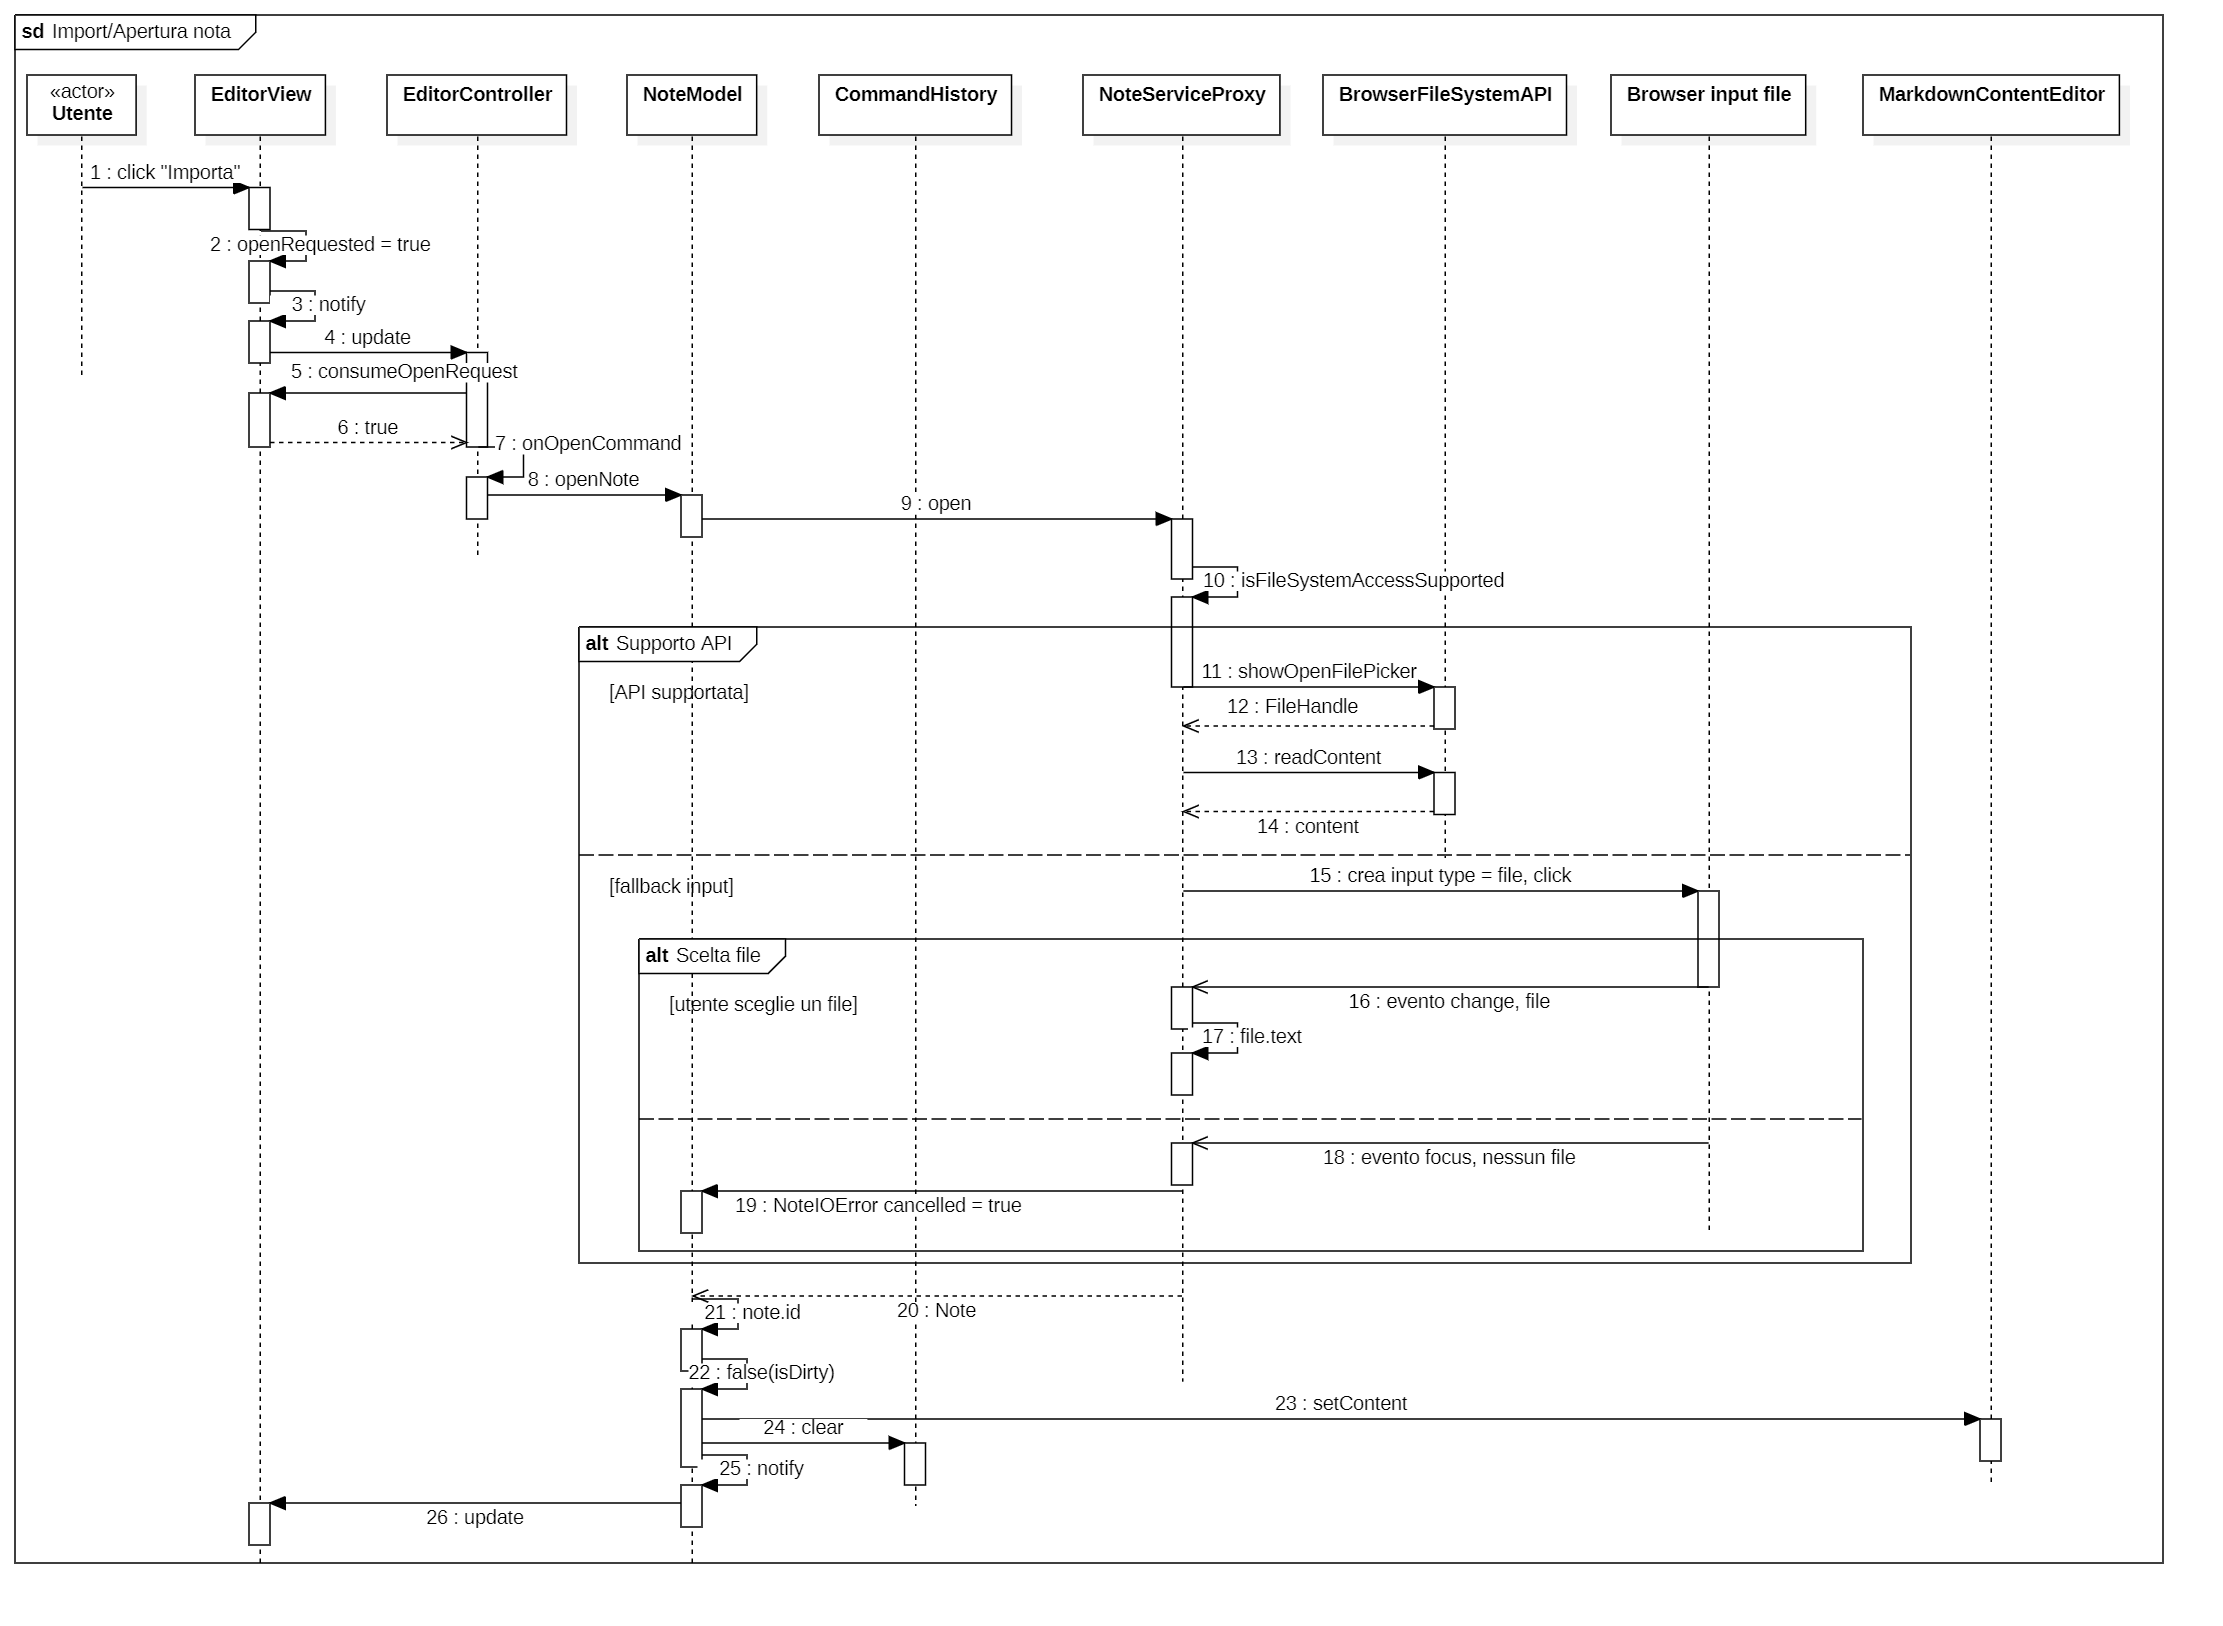
\includegraphics[width=\textwidth]{diagrammi/diagrammi_sequenze/import_apertura_nota.png}
	\caption{Importazione/Apertura di una nota esistente, con fallback per browser senza File System Access API.}
	\label{fig:seq-import}
\end{figure}

\paragraph*{Apertura nota con errore.} Speculare a ``Salvataggio con errore'': in caso di errore di I/O durante la lettura, l'eccezione \texttt{NoteIOError} risale da \texttt{BrowserFileSystemAPI} fino alla View. Un frame \texttt{alt} distingue il caso in cui l'utente ha semplicemente annullato il selettore nativo (\texttt{error.cancelled === true}), mostrato con un tono neutro non allarmante, dal caso di un vero errore di I/O, mostrato come errore.

\begin{figure}[H]
	\centering
	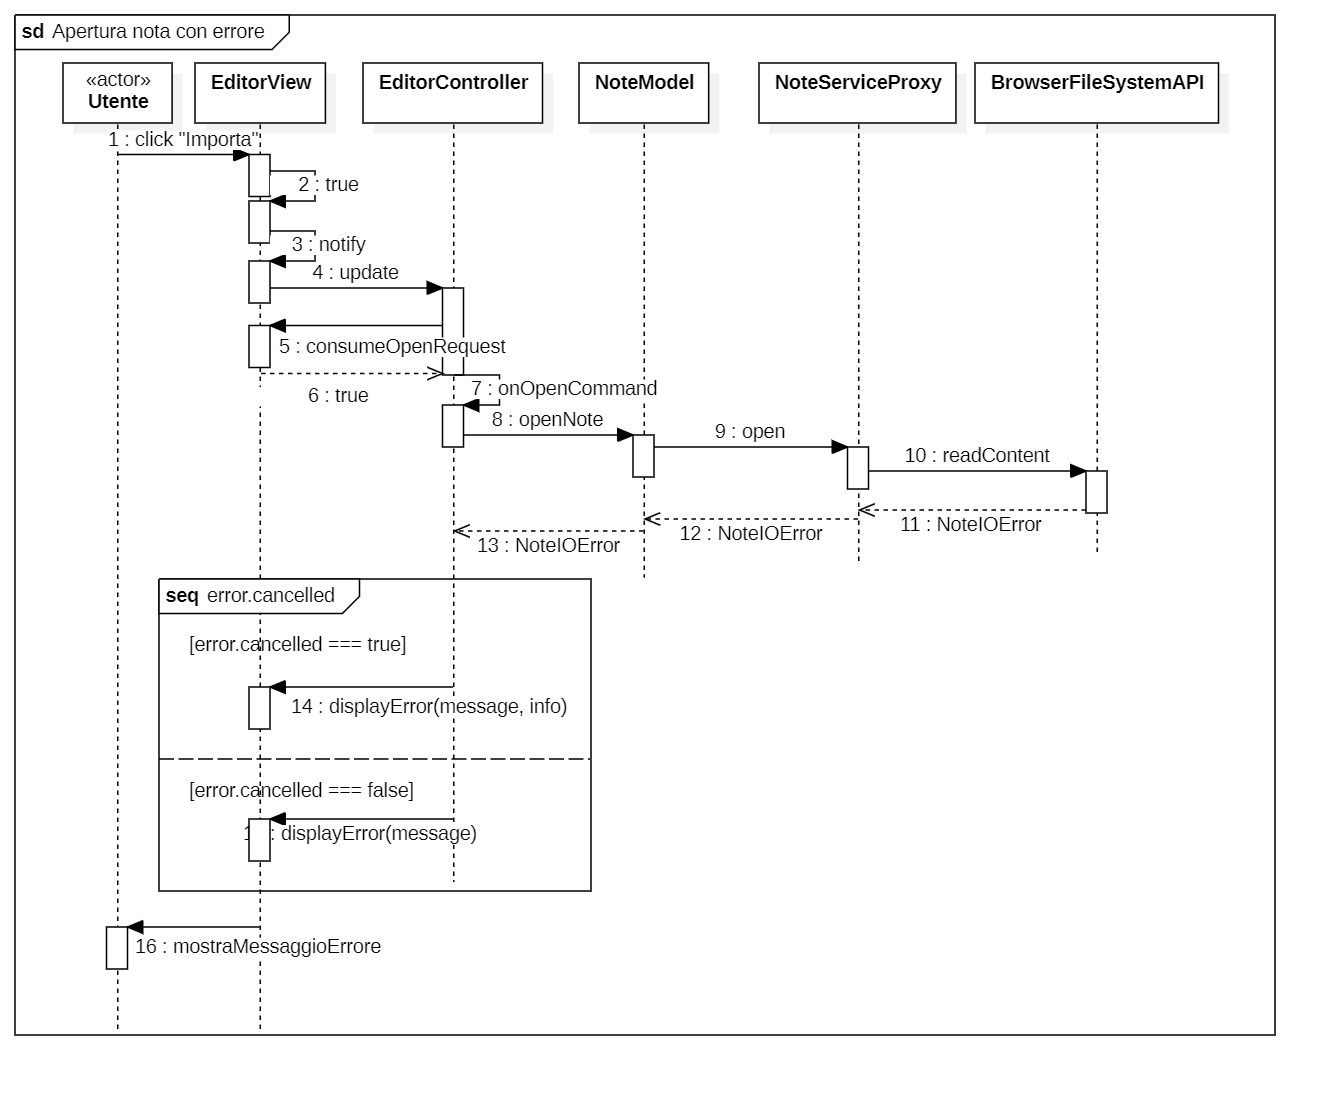
\includegraphics[width=0.85\textwidth]{diagrammi/diagrammi_sequenze/apertura_con_errore.png}
	\caption{Apertura nota con errore, con distinzione tra annullamento utente ed errore di I/O.}
	\label{fig:seq-apertura-errore}
\end{figure}

\FloatBarrier

\subsection{Esportazione}
L'esportazione della nota corrente (R77-F-O) segue un principio di indirezione controllata lato frontend, finalizzato a mantenere un accoppiamento debole tra i moduli. Al click su “Esporta”, \texttt{App.vue} delega la richiesta a \texttt{NoteModel.exportContent()}, il quale instrada la chiamata verso \texttt{ExportServiceProxy} solo se il servizio di esportazione è stato correttamente iniettato nel costruttore del Model (in caso contrario, il flusso si interrompe sollevando un'eccezione esplicita). Questa indirezione attraverso il Model, anziché una chiamata diretta della View verso il Proxy di rete, mantiene coerente il pattern di Dependency Injection adottato per tutti gli altri servizi di infrastruttura (come \texttt{NoteService} e \texttt{AIService})
\paragraph*{Export PDF (Template Method).} Il flusso di generazione segue rigorosamente lo scheletro fisso definito dalla classe astratta \texttt{Exporter} (pattern \textit{Template Method}):
\begin{itemize}
    \item Viene invocato il metodo protetto \texttt{\_prepare\_content(content)} per effettuare il parsing iniziale del Markdown e strutturare la nota nel modello intermedio di dominio \texttt{Content};
    \item Viene invocato il metodo protetto \texttt{\_convert\_format(astContent)}, l'unico passo variabile ridefinito in modo polimorfico dalla sottoclasse concreta \texttt{PdfExporter} per la compilazione in byte del file PDF finale.
\end{itemize}

\begin{figure}[H]
	\centering
	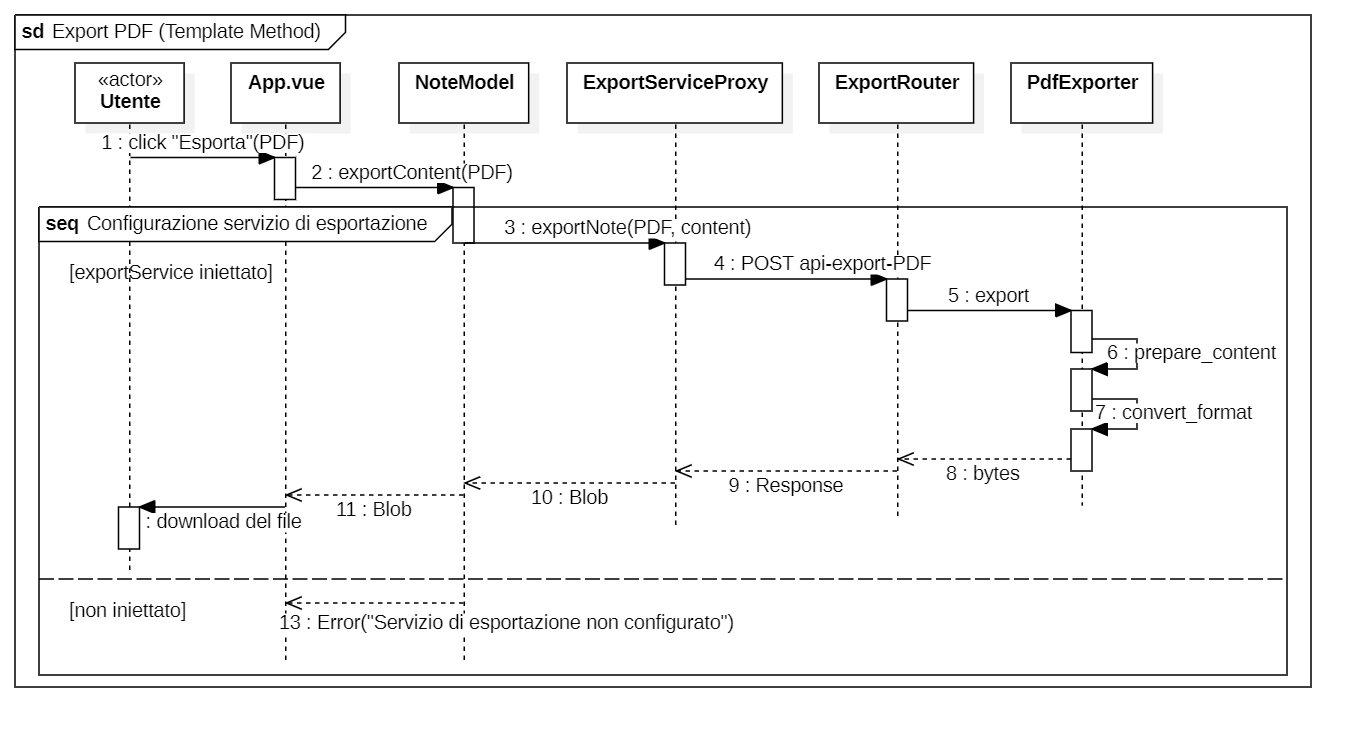
\includegraphics[width=0.9\textwidth]{diagrammi/diagrammi_sequenze/esportazione_PDF.png}
	\caption{Esportazione di una nota in PDF, dal click in \texttt{App.vue} al Template Method sul Backend.}
	\label{fig:seq-export}
\end{figure}

\FloatBarrier
